\documentclass[a4paper,12pt]{report}
\usepackage[spanish,mexico]{babel}
\usepackage[utf8]{inputenc}
\usepackage[T1]{fontenc}
\usepackage{amsmath}
\usepackage{amssymb}
\usepackage{wasysym}
\usepackage[dvipsnames,pdftex]{color}
\usepackage[colorinlistoftodos]{todonotes}
%\usepackage{helvet}
%\renewcommand{\familydefault}{\sfdefault}
\setlength{\oddsidemargin}{0in}
\usepackage{here}
\usepackage{geometry}
 \setlength{\textwidth}{6.4in}
 \setlength{\topmargin}{0in}
 \setlength{\voffset}{-0.6in}
 \setlength{\hoffset}{-0.2in}
 \setlength{\textheight}{9.7in}
 \setlength{\topskip}{0in}
 \setlength{\parskip}{2ex}
 \renewcommand{\baselinestretch}{1.5}
\usepackage{diagbox}
\usepackage{array}
\usepackage{listings}
\usepackage{caption}
%%% comandos definidos por el usuario
\begin{document}
\setcounter{page}{1}
\pagenumbering{roman}
\thispagestyle{empty}
\begin{center}
{\huge UNIVERSIDAD NACIONAL DE INGENIERÍA}\\[0.9cm]
{\Large FACULTAD DE INGENIERÍA MECÁNICA}\\[0.6in]
\end{center}
\begin{figure}[h]
\begin{center}

\includegraphics[scale=0.33]{logoUNI.png}
\vspace{0cm}
\end{center}
\end{figure}
\vspace{0.5cm}
\begin{center}
INFORME DE LABORATORIO\\
LABORATORIO DE INGENIERÍA MECÁNICA\\[14mm]
{\large MEDICIÓN DE POTENCIA EN EL COMPRESOR}\\[10mm]
\vfill
LIMA - PERÚ \hfill OCTUBRE 2019
\end{center}
\newpage
\thispagestyle{empty}
\begin{center}
{\Huge MEDICIÓN DE POTENCIA EN EL COMPRESOR}\\[0.7cm]
\small ENTREGADO:\\[0.3cm]
\small 26 OCTUBRE 2019\\[2.9cm]
\end{center}
\begin{flushleft}
{\large ALUMNOS:}\\[2cm]
\end{flushleft}
\begin{tabular}{c@{\hspace{0.5in}}c}
\rule[1pt]{2.6in}{1pt}&\rule[1pt]{2.6in}{1pt}\\
Carranza Zavala David, 20174065E & Huaroto Villavicencio Josue, 20174070I\\[2.5cm]
\rule[1pt]{2.6in}{1pt}&\rule[1pt]{2.6in}{1pt}\\
Landeo Sosa Bruno, 20172024J & Lino Carbajal Franklin, 20110146D\\[2.5cm]
\rule[1pt]{2.6in}{1pt}&\rule[1pt]{2.6in}{1pt}\\
Quesquen Vitor Angel, 20170270C & Sotelo Cavero Sergio, 20172125K\\[2.5cm]
\end{tabular}
%\begin{center}
%\begin{tabular}{c@{\hspace{0.5in}}c}
%\rule[1pt]{3.14in}{1pt}\\
%Sotelo Cavero Sergio, 20172125K% & Nombre 5, 2017 \\[1.5cm]
%\end{tabular}
%\end{center}
%\begin{center}
%\begin{tabular}{c@{\hspace{0.6in}}c}
%\rule[1pt]{3.14in}{1pt}\\
%Huaroto Villavicencio Josué, 20174070I \\[2.5cm]
%\rule[1pt]{3.14in}{1pt}\\
%Landeo Sosa Bruno, 20172024J \\[2.5cm]
%\rule[1pt]{3.14in}{1pt}\\
%Quesquen Vitor Angel, 2017 \\[2.5cm]
%\rule[1pt]{3.14in}{1pt}\\
%Sotelo Cavero Sergio, 20172125K
%\end{tabular}
%\end{center}
%\begin{center}
%\begin{tabular}{c}
%\rule[1pt]{3.14in}{1pt}\\
%Huaroto Villavicencio Josué, 20174070I \\[2.5cm]
%\end{tabular}
%\end{center}

%\rule[1pt]{3.14in}{1pt}\\
%Maguiña Amaya Wladimir, 20172019F \\[3cm]
%\rule[1pt]{3.14in}{1pt}\\
%Luis Sosa Jose, 19774147I \\[3cm]
%\rule[1pt]{3.14in}{1pt}\\
%Sotelo Cavero Sergio, 20172125K
%\end{tabular}
%\end{center}
%\\[0.7cm]
{\large PROFESOR:} \\[0.6cm]
\begin{center}
\begin{tabular}{c}
\rule[3pt]{4.8in}{1pt}\\[1pt]
ING. MORALES TAQUIRI OSWALDO
\end{tabular}
\end{center}
\vfill
%\newpage
%\begin{center}
%{\Large \bf{RESUMEN}}
%\end{center}
\newpage
\tableofcontents
%\listoffigures
%\addcontentsline{toc}{chapter}{Índice de figuras}
\newpage
\pagenumbering{arabic} %%% esto es para regresar el modo de numeración a numeración arábiga
\setcounter{page}{1}  %%% empezamos en página 1
%\part{Introducción}
\chapter{Objetivos}
\begin{enumerate}
\item Determinar la potencia indicada, al eje y potencia eléctrica del compresor de alta presión. 
\item Conocer el funcionamiento de los diferentes equipos de medición de potencia.
\item Conocer los diferentes tipos de potencia que se pueden medir en una máquina y las relaciones se pueden definir entre ellas.
\item Calcular la eficiencia mecánica del compresor de alta presión.
\end{enumerate}
\chapter{Fundamento teórico}
La energía es una magnitud almacenada, en forma similar a un volumen; su cualidad de producir trabajo o su propiedad de incrementarse, es lo único que nos interesa. La potencia es un flujo de energía, toda la energía almacenada no puede transportarse instantáneamente a otro lugar, tiene que hacerlo en forma de un flujo. Ocurre que en algunas fuentes de energía, esta no está almacenada en éste, sino que debe producirse constantemente en forma de un flujo. Por ello se habla de potencia (flujo de energía) de un motor (fuente de energía).
La energía mecánica se presenta como el producto de dos factores:
\begin{itemize}
\item El producto de una fuerza por una velocidad longitudinal: $$F \times V$$
\item El producto de un momento torsor por una Velocidad angular si el movimiento es rotacional: $$T \times \omega$$ 
\end{itemize}
La potencia se desarrolla, transmite y absorbe en máquinas rotativas y otros dispositivos. Algunas máquinas (por ejemplo, turbinas, máquinas de vapor y motores de combustión interna) desarrollan potencia. Otras la utilizan para producir efectos útiles. En todas las máquinas rotativas y alternativas hay siempre alguna forma de transmisión de potencia. En la transmisión de esta potencia, una parte de ella se pierde inevitablemente a causa de la fricción. Al ingeniero le interesa la potencia que puede desarrollarse, la que puede transmitirse y la que se utiliza para producir efectos dados. La importancia de un equipo se da por la capacidad de trabajo en la unidad de tiempo que pueda entregar.
La potencia desarrollada por la maquina no es la misma que se le da debida a las pérdidas  que se suscitan durante su funcionamiento. Sin embargo existe, una potencia entregada al pistón por la sustancia de trabajo que es determinado mediante los llamados indicadores, conociéndose esta potencia como la potencia indicada.
\chapter{Materiales}
\begin{enumerate}
\item \textbf{Tablero de control.} Controla tanto  el voltaje como la  intensidad de corriente a cada uno de los dos motores eléctricos utilizados para los compresores de alta y baja.
\item \textbf{Dos motores eléctricos.}
\item \textbf{Compresores de alta y baja presión.}
\begin{figure}[H]
\centering
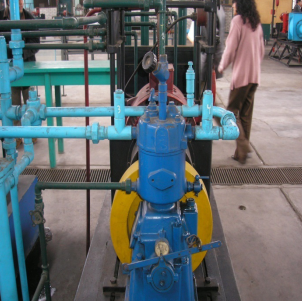
\includegraphics[scale=0.55]{Comp1.png}
\end{figure}
\begin{figure}[H]
\centering
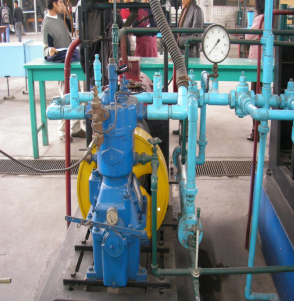
\includegraphics[scale=0.55]{Comp2.png}
\end{figure}
\item \textbf{Dinamómetro.} Permite hallar la fuerza que genera un torque equivalente al del eje del compresor.
\item \textbf{Manómetro de tipo Bourdon.} Mide las presiones tanto de salida como de la entrada.
\item \textbf{Taquímetro.} Utilizado para medir la velocidad de rotación de la volante del motor, en RPM.
\item \textbf{Contador de revoluciones tipo contador.} El número de revoluciones obtenidas por un periodo de tiempo determinado (en minutos), nos permite calcular la velocidad angular en RPM.
\item \textbf{Cronómetro digital.} Mide periodos de tiempo determinados.
\item \textbf{Tanque que almacena aire comprimido.}
\end{enumerate}
\chapter{Cálculos y resultados}
Primero ordenamos nuestras mediciones y las agrupamos en la siguiente tabla:
\begin{center}
\begin{tabular}{|c|c|c|c|}
\hline 
 & Medida 1 & Medida 2 & Medida 3 \\ 
\hline 
Voltaje CBP & 153 V & 198 V & 111 V \\ 
\hline 
Voltaje CAP & 140 V & 189 V & 165 V \\ 
\hline 
Corriente CBP & 17.5 A & 18 A & 8.8 A \\ 
\hline 
Corriente CAP & 5.5 A & 10.7 A & 17.6 A \\ 
\hline 
N CBP & 1040 RPM & 1387 RPM & 1120 RPM \\ 
\hline 
N CAP & 960 RPM & 1266 RPM & 745 RPM \\ 
\hline 
F CBP & 6.2 kgf & 6.2 kgf & 7 kgf \\ 
\hline 
F CAP & 2 kgf & 3.6 kgf & 2.35 kgf \\ 
\hline 
\end{tabular}
\end{center} 
Donde:
\begin{itemize}
\item \textbf{CBP}: Compresor Baja Presión
\item \textbf{CAP}: Compresor Alta Presión
\end{itemize}
\section{Potencia eléctrica}
$$
P = V\cdot I
$$
\begin{center}
\begin{tabular}{|c|c|c|c|}
\hline 
 & Medida 1 & Medida 2 & Medida 3 \\ 
\hline 
Potencia Eléctrica CBP & 2.6775 kW & 3.564 kW & 0.9768 kW \\ 
\hline 
Potencia Eléctrica CAP & 0.77 kW & 2.0223 kW & 2.904 kW \\ 
\hline 
\end{tabular} 
\end{center}
\section{Potencia mecánica}
$$
T = F \times r \longrightarrow P = T\cdot \frac{N}{60} \cdot 2\pi
$$
\begin{center}
\begin{tabular}{|c|c|c|c|}
\hline 
 & Medida 1 & Medida 2 & Medida 3 \\ 
\hline 
Potencia mecánica CAP & 1.6825 kW & 2.243879 kW & 2.0457257 kW\\ 
\hline 
Potencia mecánica CBP & 0.5 kW & 1.18923 kW & 0.45683 kW \\ 
\hline 
\end{tabular} 
\end{center}
\begin{figure}[H]
\centering
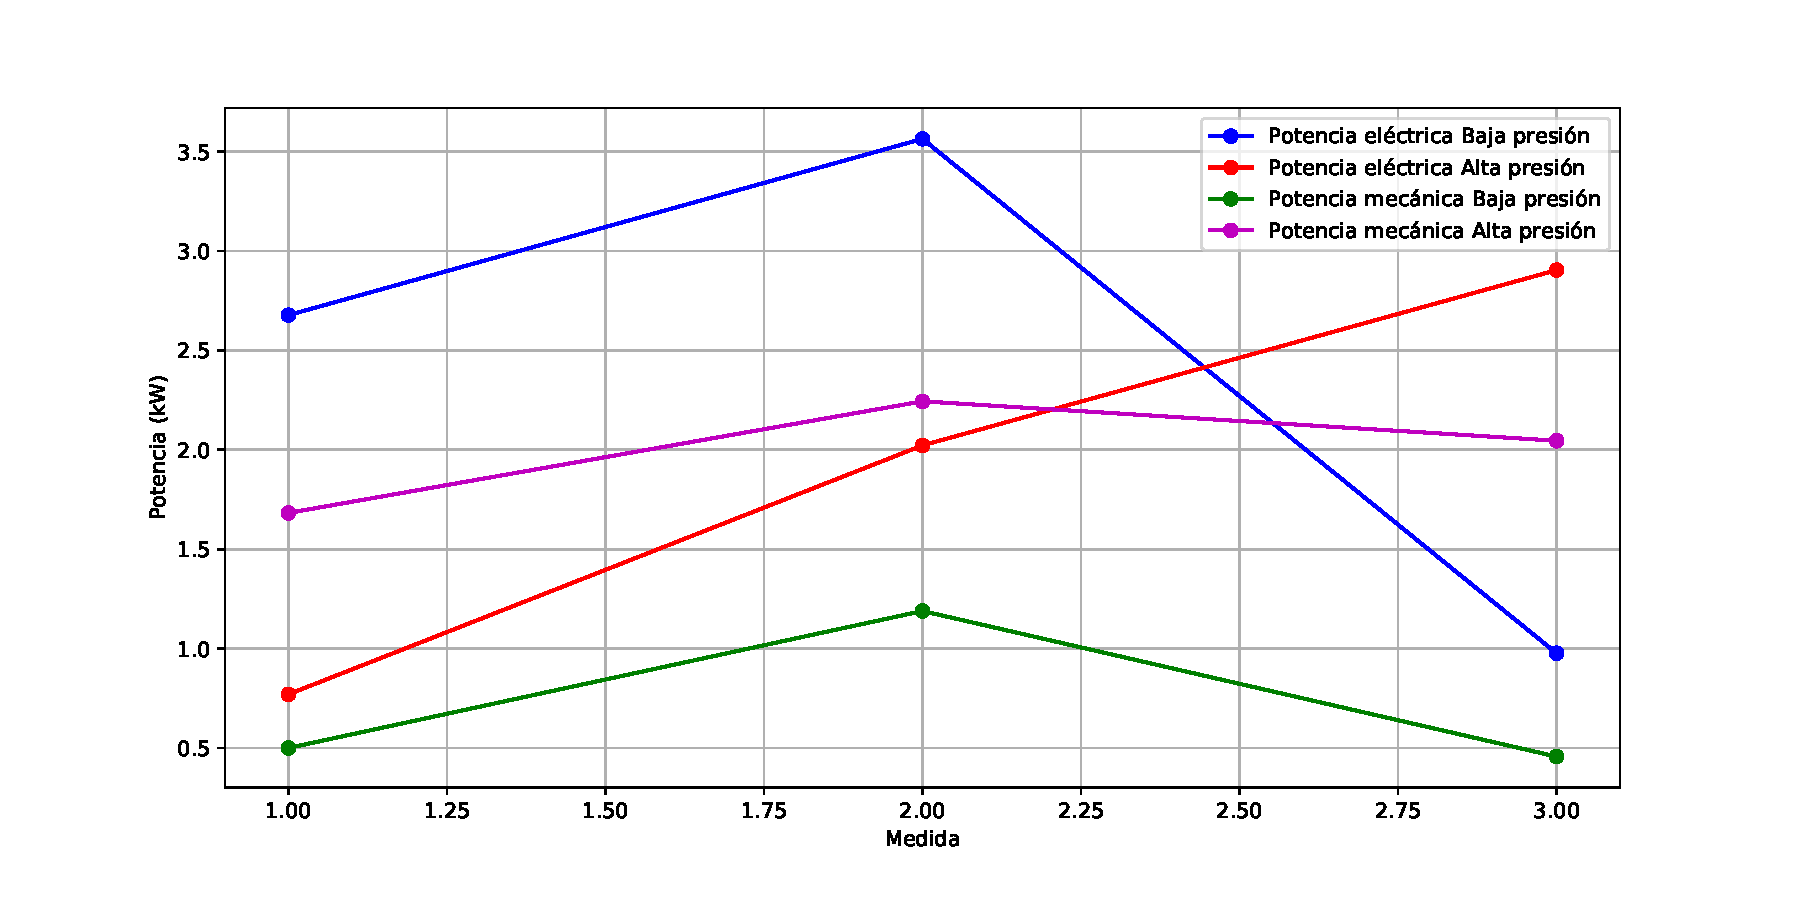
\includegraphics[scale=0.6]{potencia1.pdf}
\end{figure}
\section{Cálculo de potencia mecánica}
Considerando una eficiencia mecánica del 98\%, la potencia mecánica será:
$$
P_{m} = \frac{P}{0.98}
$$
\begin{center}
\begin{tabular}{|c|c|c|c|}
\hline 
 & Medida 1 & Medida 2 & Medida 3 \\ 
\hline 
Potencia mecánica CAP & 1.71684 kW & 2.28967 kW & 2.08747 kW\\ 
\hline 
Potencia mecánica CBP & 0.51122 kW & 1.2135 kW & 0.466154 kW \\ 
\hline 
\end{tabular} 
\end{center}
\begin{figure}[H]
\centering
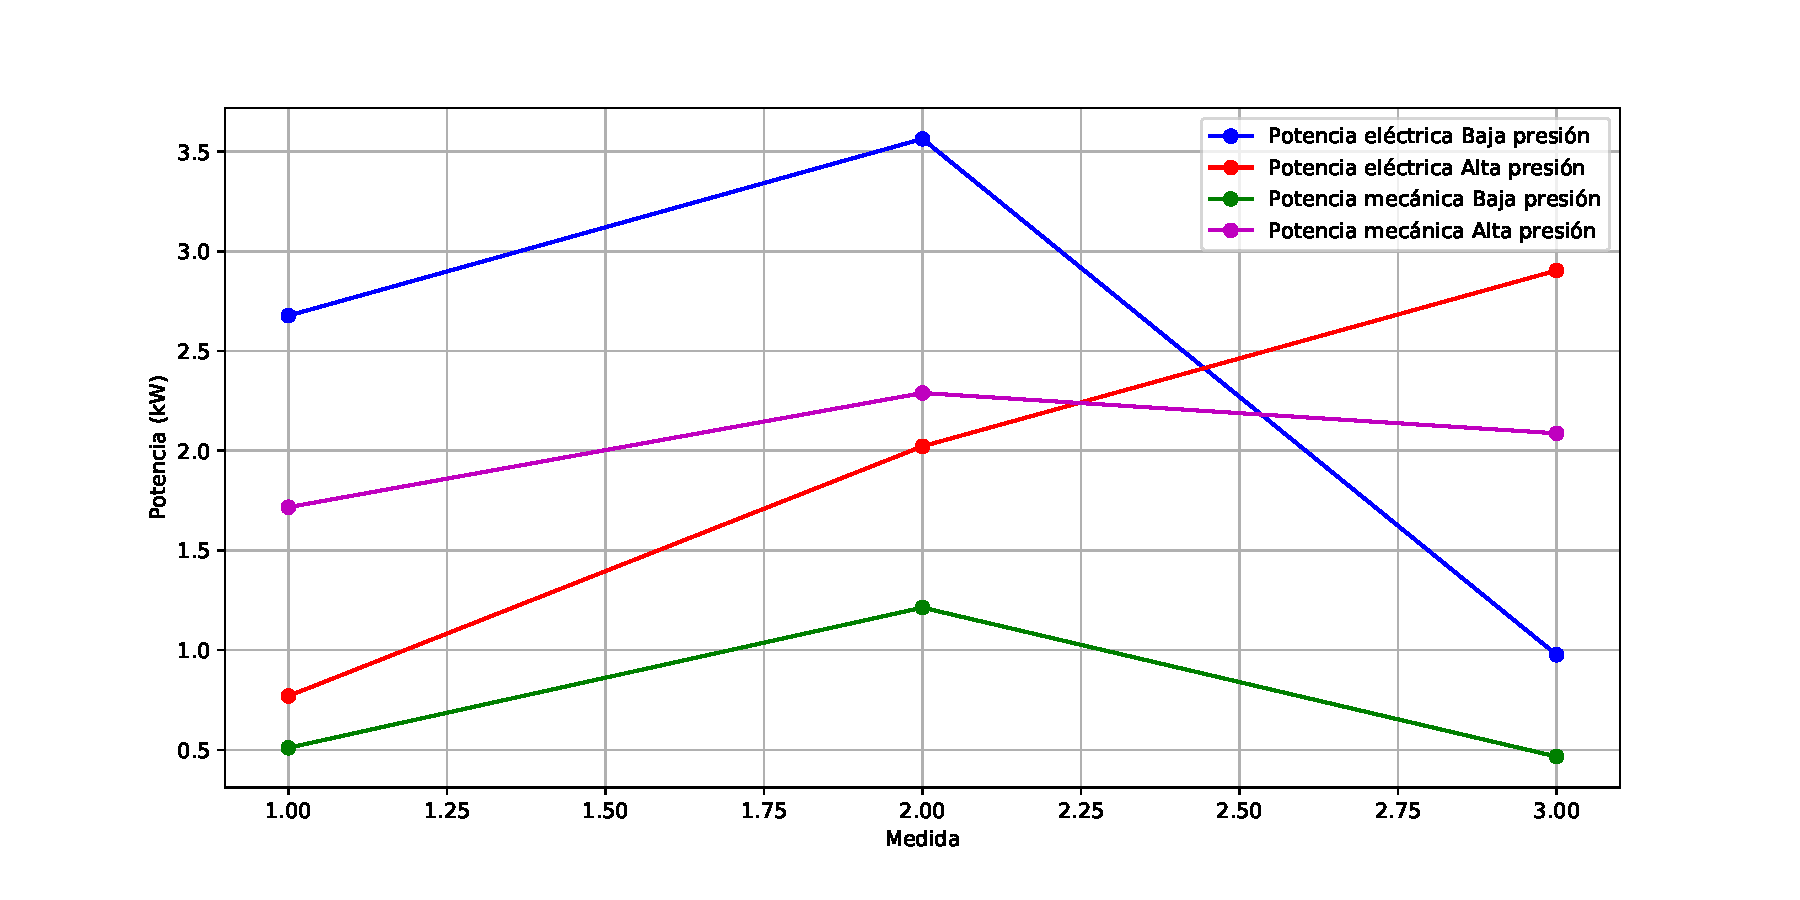
\includegraphics[scale=0.6]{potencia2.pdf}
\end{figure}
\section{Cálculo de eficiencia}
$$
e = \frac{P_{m}}{P_{e}}\cdot 100\%
$$
\begin{center}
\begin{tabular}{|c|c|c|c|}
\hline 
 & Medida 1 & Medida 2 & Medida 3 \\ 
\hline 
CBP & 18.71\% & 33.36\% & 46.76\%\\ 
\hline 
CAP & 218.51\% & 111\% & 70.44\% \\ 
\hline
\end{tabular} 
\end{center}
\begin{figure}[H]
\centering
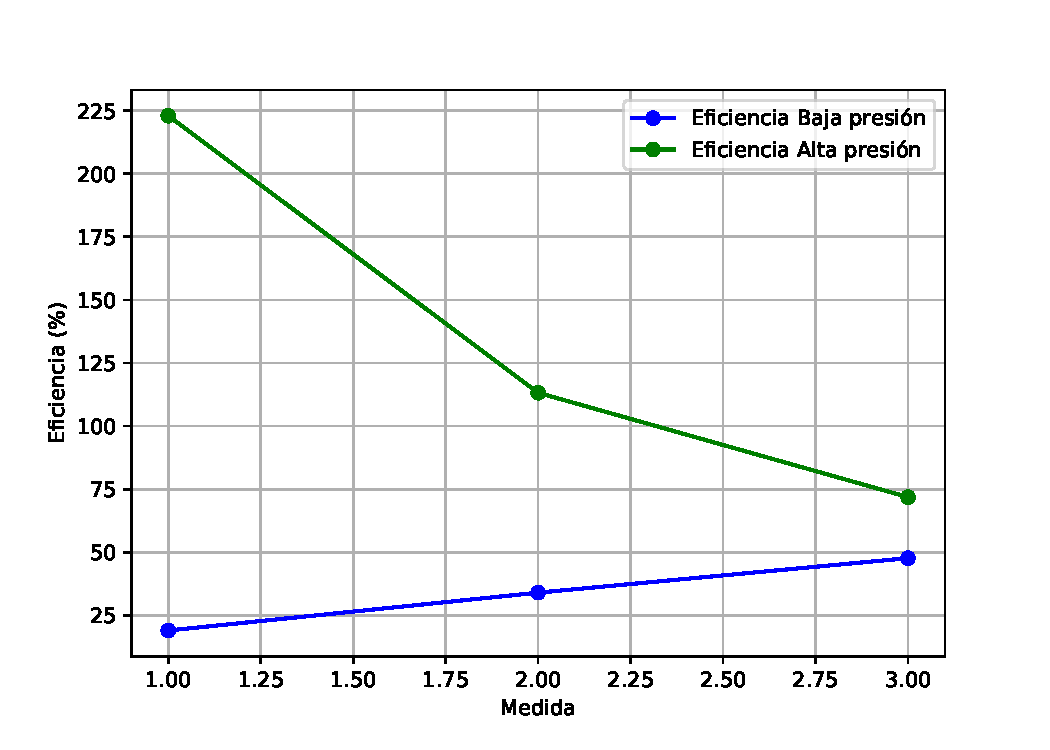
\includegraphics[scale=0.8]{eficiencia.pdf}
\end{figure}
\chapter{Conclusiones y recomendaciones}
\begin{enumerate}
\item La potencia eléctrica es mayor a la potencia al eje, debido a que siempre existen perdidas mecánicas en el motor, de esto se concluye que la eficiencia del  motor nunca es del 100\%.
\item La potencia indicada es menor que la potencia al eje. Por tal motivo la energía mecánica que se tiene que entregar al eje del compresor es mayor que la necesaria para la compresión, en el valor de las pérdidas mecánicas.
\item La potencia eléctrica indicada y al eje guardan una relación directamente proporcional con las RPM.
\item La presión media indicada depende del área del ciclo termodinámico así como la longitud del diagrama y de la constante del resorte.
\item Realizamos regulaciones de voltaje y de corriente.
\item Realizamos la toma de  nuestros datos del laboratorio, cuando la presión del tanque de almacenamiento de aire era constante.
\end{enumerate}
\begin{thebibliography}{99}  %%%este es un contador para el número de bibliografías utilizados.
\addcontentsline{toc}{chapter}{Bibliograf\'{\i}a} %%% Para introducir la bibliografía en el índice.
%\bibitem{Rahman}{Rahman,Aminur y Doe, Hidekazu; ``Ion transfer of tetraalkylammonium cations at an interface between 
%frozen aqueous solution and 1,2-dichloroethane".{\em{Journal of Electroanalytical Chemistry}} {\bfseries 424},159,(1997).}
\bibitem{Gro}{Chow, V.``Open Channel Hydraulics''.{\em{McGraw-Hill}}}
\bibitem{Gro}{Domínguez, F.``Hidráulica''.}
\bibitem{Ding}{Guevara, Robert (2009).``Manual de prácticas de laboratorio de energía II''.}
\bibitem{AL}{Mott, R. ``Mecánica de fluidos''.\em{Prentice-Hall}}
%\bibitem{AL}{Alonso, Jose M. ``Técnicas de mecanizado 1". {\em{Paraninfo}} {\bfseries España-Madrid}, 6-20, (2001).}
%\bibitem{Samec2}{Samec Z., Lhotsky A., Jänchenová H., y Marecek, V. ``Interfacial tension and impedance measurements
%of interfaces between two inmiscible electrolyte solutions". {\em{Journal of Electroanalytical Chemistry}} {\bfseries
%43}, 47, (2000).}
%\bibitem{Day}{Day R.A. y Underwood A.L. {\textit{Química Analítica Cuantitativa}},5ºed. Prentice-Hall, México, 1998. 45-48.}
%\bibitem{Keyser}{Farah Abud, Michel. ``Determinación de la vida útil en herramientales de corte endurecido por el proceso de borurización en pasta''. {\em{Instituto tecnológico y de estudios superiores de Monterrey}}}
%\bibitem{Zolotorevski}{Escalona, I. ``Máquinas: herramientas por arranque de viruta.''.{\em{El Cid Editor.}}}
%\bibitem{Lasheras}{Lasheras. ``Tecnología de los Materiales Industriales''.} 
%\bibitem{Dieter}{Dieter. ``Metalurgia mecánica''.}
%\bibitem{Apraiz}{Apraiz, J. ``Tratamiento Térmico de los Aceros''.}
%\bibitem{Smith}{Smith, William F. y Ph.D. Hashemi, Javad ``Ciencia e ingeniería de materiales". {\em{
%Madrid: McGraw-Hill, Interamericana de España.}} 570, (2004).} 
%\bibitem{Callister}{Callister, William D. y Rethwisch, David G. ``Introducción a la ingeniería de los materiales''. %{\em{Barcelona Reverté.}}, 960, (2007).} 
%\bibitem{Askeland}{Askeland, Donald R., Pradeep P. Phulé y Wright, Wendelin J. ``Ciencia e ingeniería de los materiales''.{\em{México, D.F. Internacional Thomson Editores.}} {\textit{$6^{ta}$ edición}}, 1004, (2012).}
%\bibitem{HARDBANDING}{Tabla de conversión de escala de durezas. \begin{verbatim}http://%hardbandingsolutions.com/postle_sp/hardness.php
%\end{verbatim}}
%\bibitem{PR}{Termómetro bimetálico. \begin{verbatim}
%https://www.electrabel.es/el-funcionamiento-de-un-termometro-bimetalico/\end{verbatim}}
%\bibitem{PR}{Termómetro de inmersión total. \begin{verbatim}
%http://www.dilabsa.com/es/cual-es-la-diferencia-entre-los-termometros-
%de-inmersion-total-y-parcial/
%\end{verbatim}}
%\bibitem{PR}{Termómetro de inmersión parcial. \begin{verbatim}
%http://www.metas.com.mx/guiametas/La-Guia-MetAs-08-09-termometros-liquido-
%en-vidrio.pdf
%\end{verbatim}}
%\bibitem{HE}{Fresadora. \begin{verbatim} http://lizdenbow.blogspot.com/
%\end{verbatim}}
%\bibitem{ASTM}{Normas ASTM.}
%\bibitem{NTP}{Normas NTP.}
\end{thebibliography}
\end{document}